% MagistralaCAN4_doc_extended.tex
% Kompilacja: pdflatex -> pdflatex (dla spisu treści i referencji)
\documentclass[a4paper,12pt,polish]{article}
\usepackage[T1]{fontenc}
\usepackage[utf8]{inputenc}
\usepackage{babel}
\usepackage{geometry}
\geometry{margin=2.5cm}
\usepackage{hyperref}
\usepackage{graphicx}
\usepackage{tikz}
\usetikzlibrary{shapes.geometric, arrows, positioning, calc, fit, backgrounds, chains, scopes}
\usepackage{listings}
\usepackage{xcolor}
\usepackage{booktabs}
\usepackage{caption}
\usepackage{float}
\usepackage{enumitem}
\usepackage{fancyhdr}
\usepackage{pgfplots}
\pgfplotsset{compat=1.18}
\usepackage{longtable}
\usepackage{array}
\usepackage{multirow}
\usepackage{makecell}
\usepackage{amssymb}

% Kolorystyka cyberpunk
\definecolor{bgdark}{HTML}{0a0e17}
\definecolor{neongreen}{HTML}{00ffaa}
\definecolor{neonpink}{HTML}{ff66cc}
\definecolor{neonorange}{HTML}{ffaa00}
\definecolor{accent}{HTML}{e94560}
\definecolor{codebg}{HTML}{1a1a2e}

\lstset{
  basicstyle=\ttfamily\small\color{white},
  backgroundcolor=\color{codebg},
  frame=single,
  rulecolor=\color{accent},
  keywordstyle=\color{neongreen},
  commentstyle=\color{neonpink},
  stringstyle=\color{neonorange},
  showstringspaces=false,
  numbers=left,
  numberstyle=\tiny\color{gray},
  breaklines=true,
  captionpos=b
}

\title{\textbf{MagistralaCAN4}\\[0.2cm] \large Wysokowydajny sniffer CAN z uczeniem asocjacyjnym i skryptami Lua}
\author{Dokumentacja techniczna – wersja rozszerzona}
\date{\today}

\pagestyle{fancy}
\fancyhf{}
\fancyhead[L]{\small MagistralaCAN4 -- dokumentacja}
\fancyhead[R]{\small Wersja 2.0}
\fancyfoot[C]{\thepage}
\renewcommand{\headrulewidth}{0.4pt}

\begin{document}

\maketitle
\thispagestyle{empty}
\vspace{2cm}
\begin{center}
\textit{Narzędzie do analizy i diagnostyki magistrali CAN/CAN FD}\\
\vspace{0.5cm}

\includegraphics[width=0.4\textwidth]{ico.png} % placeholder for logo
\end{center}
\newpage

\tableofcontents
\newpage

% ======================================================================
\section{Wprowadzenie}
\label{sec:intro}

\textbf{MagistralaCAN4} jest zaawansowanym, wielowątkowym narzędziem dla inżynierów pracujących z magistralami CAN i CAN FD. Powstało z myślą o szybkiej identyfikacji zależności pomiędzy zdarzeniami fizycznymi (np. naciśnięcie hamulca) a ruchem na magistrali, przy jednoczesnym zapewnieniu maksymalnej wydajności dzięki wykorzystaniu GPU oraz intuicyjnego interfejsu użytkownika.

Główne możliwości:
\begin{itemize}[noitemsep]
  \item \textbf{Przechwytywanie ramek} CAN 2.0 i CAN FD z interfejsów socketCAN z nadpisywaniem lub dopisywaniem.
  \item \textbf{Uczenie asocjacyjne} oparte na analizie okien czasowych, kontraście ze zdarzeniami tła, korelacjach liniowych i nieliniowych (Pearson, Mutual Information, MIC), regresji liniowej, łańcuchach Markowa, k-średnich, PCA oraz automatycznej detekcji zdarzeń.
  \item \textbf{Silnik skryptowy Lua} umożliwiający automatyzację reakcji na ramki (wysyłanie, logowanie) poprzez API \texttt{sendFrame}, \texttt{log}, \texttt{getTick}.
  \item \textbf{Obsługa plików DBC} – parsowanie, wyświetlanie nazwanych sygnałów w widoku szczegółów ramki oraz dashboard na żywo z aktualnymi wartościami.
  \item \textbf{Analiza offline} – wczytywanie plików \texttt{candump} z odtwarzaniem z oryginalnymi znacznikami czasu, trybem krokowym i pełną integracją z modułem uczenia.
  \item \textbf{Eksport} do formatu \texttt{candump}, modeli asocjacyjnych (JSON) oraz automatyczne generowanie skryptów Lua na podstawie wyuczonych reguł.
  \item \textbf{Interaktywny edytor bajtów} w widoku ramki z możliwością wysyłania zmodyfikowanych ramek.
  \item \textbf{Powiadomienia systemowe} (tray) oraz globalne skróty klawiszowe (Ctrl+Shift+E dla zdarzenia).
\end{itemize}

Projekt jest rozwijany w C++17 z wykorzystaniem Qt6, OpenCL oraz Lua. Architektura oparta jest na osobnych wątkach dla akwizycji i interfejsu, a obliczenia mogą być akcelerowane przez GPU. Kod źródłowy podzielony jest na czytelne moduły, co ułatwia dalszy rozwój.

\section{Architektura systemu}
\label{sec:arch}

\subsection{Ogólny schemat blokowy}
Poniższy diagram (rys.~\ref{fig:arch}) przedstawia główne bloki funkcjonalne aplikacji wraz z przepływem danych.

\begin{figure}[H]
\centering
\begin{tikzpicture}[
  block/.style={rectangle, rounded corners, draw=accent, fill=codebg, text=white, minimum width=2.8cm, minimum height=0.9cm, font=\small\bfseries},
  data/.style={rectangle, draw=neongreen, fill=codebg, text=neongreen, minimum width=2.4cm, minimum height=0.8cm, font=\small},
  arrow/.style={->, >=stealth, thick, color=neonorange},
  line/.style={draw=accent, thick}
]
% Warstwy
\begin{pgfonlayer}{background}
\node[fit={(0,0) (14,-10)}, fill=bgdark!50, rounded corners, label=above:{\textbf{MagistralaCAN4}}] {};
\end{pgfonlayer}

% Warstwa interfejsu
\node[block] (gui) at (2, -1) {GUI (Qt6)};
\node[block, right=3cm of gui] (toolbar) {Pasek narzędzi};
\node[block, right=3cm of toolbar] (tabs) {Zakładki};
% Warstwa logiki
\node[block, below=2cm of gui] (sniffer) {CanSniffer (wątek)};
\node[block, right=3cm of sniffer] (model) {CanFrameModel};
\node[block, below=2cm of sniffer] (learner) {AssociativeLearner};
\node[block, right=3cm of learner] (lua) {LuaScriptEngine};
\node[block, below=2cm of learner] (offline) {OfflineAnalyzer};
\node[block, right=3cm of offline] (dbc) {DbcParser + LiveDashboard};
\node[block, left=3cm of offline] (detail) {FrameDetailWidget};
% Warstwa sprzętowa
\node[data, below=2cm of offline, xshift=2cm] (can) {Interfejs CAN (socket)};

% Połączenia
\draw[arrow] (sniffer) -- node[above, font=\tiny] {CanFrame} (model);
\draw[arrow] (sniffer) |- (learner);
\draw[arrow] (sniffer) |- (lua);
\draw[arrow] (sniffer) |- (dbc);
\draw[arrow] (gui) -- (sniffer) node[midway, left, font=\tiny] {start/stop};
\draw[arrow] (model) -- (detail) node[midway, left, font=\tiny] {klik};
\draw[arrow] (learner) -- (offline) node[midway, left, font=\tiny] {zdarzenia};
\draw[arrow] (dbc) -- (detail) node[midway, right, font=\tiny] {sygnały};
\draw[arrow] (can) -- (sniffer) node[midway, right, font=\tiny] {ramki};
\draw[arrow] (toolbar) -- (gui);
\draw[arrow] (tabs) -- (gui);
\draw[line, dashed] (learner) -- node[above, font=\tiny, text=white] {OpenCL} ++(2,0);
\end{tikzpicture}
\caption{Ogólny schemat blokowy systemu MagistralaCAN4.}
\label{fig:arch}
\end{figure}

\subsection{Warstwy systemu}
Aplikację można podzielić na trzy logiczne warstwy:
\begin{enumerate}[noitemsep]
  \item \textbf{Warstwa interfejsu użytkownika} – odpowiada za prezentację danych (tabele, wykresy, dashboard) oraz interakcję z operatorem. Wykorzystuje Qt6 Widgets, Charts oraz QSystemTrayIcon dla powiadomień.
  \item \textbf{Warstwa logiki} – zawiera moduły analityczne (uczenie asocjacyjne, statystyka, Lua) oraz zarządzanie danymi. Tutaj wykonywane są obliczenia, również z wykorzystaniem GPU (OpenCL) i wielowątkowości CPU (QtConcurrent).
  \item \textbf{Warstwa komunikacji} – odpowiada za odczyt i zapis ramek CAN poprzez gniazda socketCAN. Uruchamiana jest w osobnym wątku, aby nie blokować GUI.
\end{enumerate}

\subsection{Przepływ danych}
Rysunek~\ref{fig:dataflow} przedstawia szczegółowy przepływ ramek od magistrali do poszczególnych konsumentów.

\begin{figure}[H]
\centering
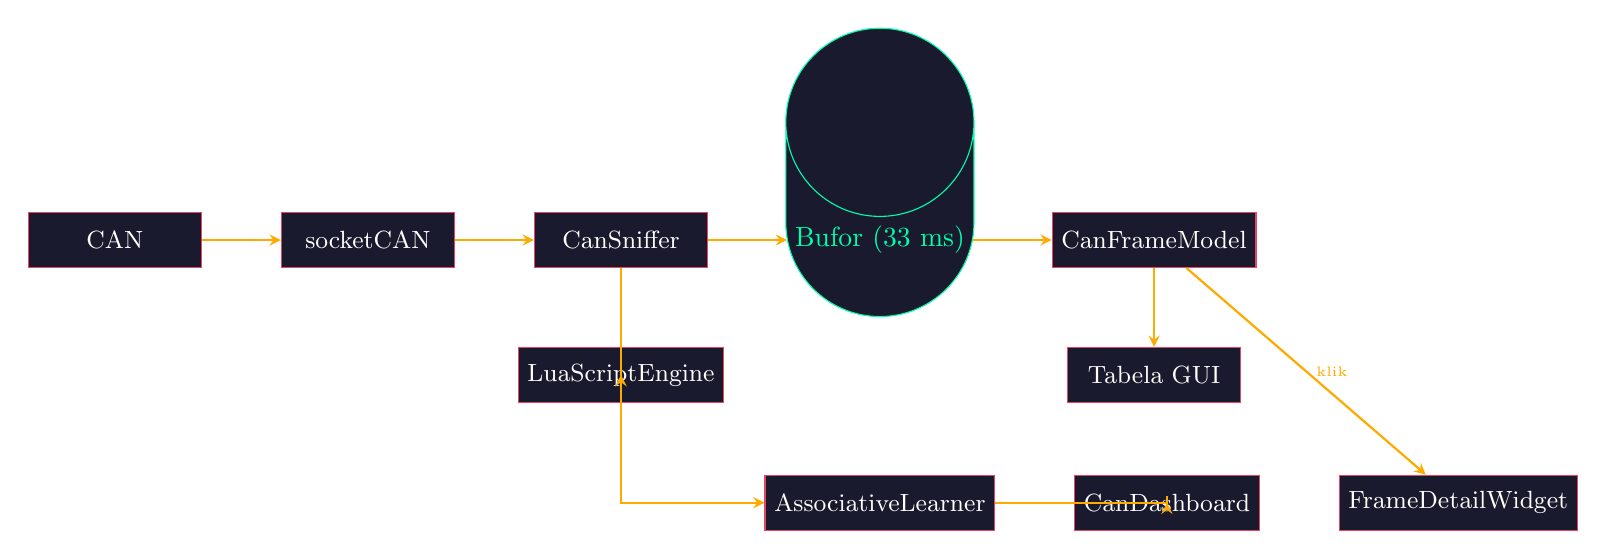
\begin{tikzpicture}[
  block/.style={rectangle, draw=accent, fill=codebg, text=white, minimum width=2.2cm, minimum height=0.7cm, font=\small},
  queue/.style={cylinder, draw=neongreen, fill=codebg, text=neongreen, shape border rotate=90, minimum width=1.8cm, minimum height=1cm},
  arrow/.style={->, >=stealth, thick, color=neonorange}
]
\node[block] (can) {CAN};
\node[block, right=1cm of can] (socket) {socketCAN};
\node[block, right=1cm of socket] (sniffer) {CanSniffer};
\node[queue, right=1cm of sniffer] (buf) {Bufor (33 ms)};
\node[block, right=1cm of buf] (model) {CanFrameModel};
\node[block, below=1cm of model] (table) {Tabela GUI};
\node[block, below=1cm of sniffer] (lua) {LuaScriptEngine};
\node[block, below=2cm of buf] (learner) {AssociativeLearner};
\node[block, right=1cm of learner] (dashboard) {CanDashboard};
\node[block, right=1cm of dashboard] (detail) {FrameDetailWidget};
\draw[arrow] (can) -- (socket);
\draw[arrow] (socket) -- (sniffer);
\draw[arrow] (sniffer) -- (buf);
\draw[arrow] (buf) -- (model);
\draw[arrow] (model) -- (table);
\draw[arrow] (sniffer) |- (lua);
\draw[arrow] (sniffer) |- (learner);
\draw[arrow] (learner) -| (dashboard);
\draw[arrow] (model) -- (detail) node[midway, right, font=\tiny] {klik};
\end{tikzpicture}
\caption{Przepływ danych w systemie.}
\label{fig:dataflow}
\end{figure}

Ramki z magistrali są odczytywane w wątku CanSniffer i emitowane przez sygnał \texttt{newFrame}. Główny wątek buforuje je przez 33 ms, po czym wsadowo aktualizuje model tabeli. Równolegle te same ramki trafiają do modułów asocjacyjnego, Lua oraz dashboardu.

\section{Opis modułów}
\label{sec:modules}

\subsection{CanSniffer}
Klasa odpowiada za otwarcie gniazda CAN RAW (z obsługą CAN FD) oraz odczyt ramek w pętli nieskończonej. Uruchamiana w osobnym wątku przez \texttt{QtConcurrent::run}. Ramki są parsowane do struktury \texttt{CanFrame} i emitowane jako sygnał. Obsługuje również wysyłanie ramek (\texttt{writeFrame}) wykorzystywane przez Lua i edytor.

\subsection{CanFrameModel}
Model tabeli dziedziczący po \texttt{QAbstractTableModel}. Przechowuje listę ramek (z opcjonalnym nadpisywaniem wg ID) i aktualizuje widok w trybie wsadowym co 33 ms, co zapewnia wysoką wydajność przy dużym obciążeniu.

\subsection{AssociativeLearner}
Centralny moduł analityczny. Udostępnia szereg analiz:
\begin{itemize}[noitemsep]
  \item \textbf{Lista kandydatów} – identyfikatory CAN pojawiające się we wszystkich zdarzeniach; ranking na podstawie podobieństwa wektorów cech.
  \item \textbf{Korelacja wartość--bajt} – współczynniki Pearsona między wprowadzaną zmienną (np. temperatura) a bajtami ramek.
  \item \textbf{Sekwencje} – najczęstsze bigramy i trigramy ID w oknach zdarzeń.
  \item \textbf{Korelacja międzybajtowa} – zależności między bajtami różnych identyfikatorów.
  \item \textbf{Mutual Information (MI)} – nieliniowa miara zależności.
  \item \textbf{MIC (Maximal Information Coefficient)} – znormalizowana (0–1) miara zdolna wykryć dowolne zależności.
  \item \textbf{Predykcja wartości} – regresja liniowa dla silnie skorelowanych bajtów, bieżąca prognoza zmiennej.
  \item \textbf{Predykcja sekwencji (Markov)} – na podstawie historii ramek przewiduje najbardziej prawdopodobne następne ID.
  \item \textbf{Detekcja anomalii} – buduje model normalny i sygnalizuje odchylenia.
  \item \textbf{Auto-detekcja zdarzeń} – monitoruje gradient zmiennej i korelacje, automatycznie rejestruje zdarzenia.
  \item \textbf{Klastrowanie (k-średnich)} – grupuje okna ramek w stany magistrali.
  \item \textbf{PCA + k-średnich} – redukcja wymiarów do 2D, wizualizacja klastrów.
  \item \textbf{Macierz korelacji zmiennych} – heatmapa zależności między wszystkimi zmiennymi.
  \item \textbf{Eksport/import modeli} – zapis i odczyt wyuczonych parametrów (JSON).
  \item \textbf{Generator skryptów Lua} – tworzy reguły na podstawie najlepszych kandydatów.
\end{itemize}

\subsection{GpuCorrelator}
Klasa wykorzystująca OpenCL do szybkiego obliczania macierzy korelacji (iloczyn skalarny). W przypadku braku GPU przełącza się na wielowątkowy CPU.

\subsection{LuaScriptEngine}
Silnik Lua z predefiniowanymi funkcjami: \texttt{sendFrame(id, data\_table)}, \texttt{log("tekst")}, \texttt{getTick()}. Wczytuje pliki \texttt{.lua} zawierające funkcję \texttt{onFrame(id, data, timestamp)}.

\subsection{DbcParser i CanDashboard}
Parser plików DBC ekstrahuje definicje wiadomości i sygnałów. Dashboard wyświetla aktualne wartości sygnałów w czasie rzeczywistym na podstawie ostatnich ramek.

\subsection{OfflineAnalyzer}
Umożliwia wczytanie pliku \texttt{candump}, odtwarzanie z oryginalnymi odstępami czasu (regulowana prędkość), tryb krokowy (Enter) oraz integrację z modułem asocjacyjnym.

\subsection{FrameDetailWidget}
Widok szczegółów ramki: identyfikator, DLC, czas, siatka 8×8 bitów z podświetlaniem zmian. Po wczytaniu DBC wyświetla nazwy sygnałów. Tryb edycji pozwala zmieniać bajty i bity, a następnie wysłać zmodyfikowaną ramkę.

\subsection{CandidateModel}
Prosty model listy kandydatów (CAN ID, opis, pewność, wystąpienia) używany przez AssociativeLearner.

\subsection{Logger}
Zapisuje zdarzenia (z timestampem) do \texttt{~/magistrala\_can4.log} oraz wypisuje na konsolę.

\section{Interfejs użytkownika}
\label{sec:gui}

\subsection{Pasek narzędzi}
Zawiera:
\begin{itemize}[noitemsep]
  \item ComboBox z listą dostępnych interfejsów CAN (odświeżanie przyciskiem ↻),
  \item Przycisk Start/Stop,
  \item Checkbox nadpisywania ramek,
  \item Etykieta statusu,
  \item Akcje: Wyczyść, Eksportuj candump, Wczytaj Lua, Wczytaj DBC.
\end{itemize}

\subsection{Zakładki}
\begin{enumerate}[noitemsep]
  \item \textbf{Ruch CAN} – tabela z kolumnami: CAN ID, Typ (STD/EXT), RTR, DLC, Dane (hex), Czas.
  \item \textbf{Uczenie asocjacyjne} – przewijalny panel z polami do zarządzania zmiennymi i przyciskami akcji oraz licznymi tabelami wyników i wykresami.
  \item \textbf{Szczegóły ramki} – interaktywna siatka bajtów/bitów.
  \item \textbf{Analiza offline} – kontrolki do wczytywania i odtwarzania plików.
  \item \textbf{Dashboard CAN} – panele z aktualnymi wartościami sygnałów DBC.
\end{enumerate}

\subsection{Skróty klawiszowe}
\begin{itemize}[noitemsep]
  \item \texttt{Ctrl+Shift+E} -- zarejestruj zdarzenie,
  \item \texttt{Ctrl+Shift+D} -- zarejestruj brak zdarzenia,
  \item \texttt{Enter} – w trybie offline odtwarza następną ramkę.
\end{itemize}

\subsection{Powiadomienia systemowe}
Aplikacja wyświetla dymki systemowe przy zdarzeniach asocjacyjnych i anomaliach. Ikona w tray'u umożliwia szybki dostęp.

\section{Uczenie asocjacyjne – przewodnik}
\label{sec:learning}

\subsection{Przygotowanie danych}
Należy wybrać (lub dodać) zmienną liczbową (np. temperatura, obroty) i wprowadzać jej wartości w momencie obserwacji. Program przechowuje wartości wraz ze średnimi bajtami ramek z okna czasowego (±500 ms, adaptacyjne).

\subsection{Analiza zdarzeń i tła}
Kliknięcie \texttt{�� Zarejestruj zdarzenie} zapamiętuje bieżące okno ramek jako zdarzenie. Kliknięcie \texttt{⛔ Brak zdarzenia} zapisuje okno jako tło. Algorytm porównuje cechy ID pomiędzy zdarzeniami a tłem – im bardziej ID przypomina tło, tym jego punktacja jest obniżana.

\begin{figure}[H]
\centering
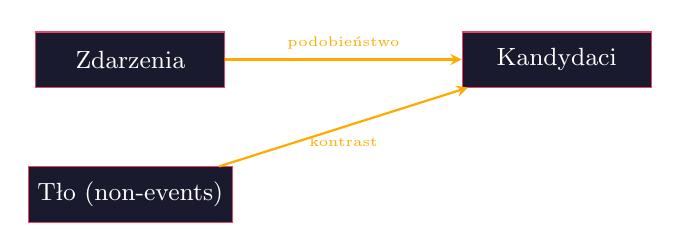
\begin{tikzpicture}[
  box/.style={rectangle, draw=accent, fill=codebg, text=white, minimum width=2.4cm, minimum height=0.7cm, font=\small},
  arrow/.style={->, >=stealth, thick, color=neonorange}
]
\node[box] (ev) {Zdarzenia};
\node[box, below=1cm of ev] (bg) {Tło (non-events)};
\node[box, right=3cm of ev] (cand) {Kandydaci};
\draw[arrow] (ev) -- node[above, font=\tiny] {podobieństwo} (cand);
\draw[arrow] (bg) -- node[below, font=\tiny] {kontrast} (cand);
\end{tikzpicture}
\caption{Wpływ zdarzeń i tła na listę kandydatów.}
\label{fig:contrast}
\end{figure}

\subsection{Korelacje, MI i MIC}
Po zebraniu co najmniej 3 obserwacji można obliczyć:
\begin{itemize}[noitemsep]
  \item \textbf{Korelację Pearsona} – standardową miarę liniową.
  \item \textbf{Mutual Information} – opartą na entropii, wykrywa nieliniowości.
  \item \textbf{MIC} – znormalizowaną miarę odporną na typ zależności.
\end{itemize}
Wyniki prezentowane są w tabelach z kolorowaniem (zielony – silna zależność).

\subsection{Predykcja i sekwencje}
Regresja liniowa tworzy model \texttt{y = a·x + b} dla każdej pary (ID, bajt) o wysokiej korelacji. Co 500 ms aktualizowana jest prognoza wartości zmiennej. Łańcuch Markowa zlicza przejścia między ID i wyświetla najbardziej prawdopodobny następny identyfikator.

\subsection{Klastrowanie i PCA}
K-średnich (K=3 domyślnie, z opcją automatycznego doboru metodą łokcia) grupuje okna czasowe w stany magistrali. PCA redukuje wymiar do 2D i umożliwia wizualizację (rys.~\ref{fig:pca}).

\subsection{Eksport modeli i reguł Lua}
Wyuczone modele (parametry regresji, łańcuch Markowa, model normalny) można zapisać do JSON i później wczytać. Przycisk \texttt{�� Generuj skrypt Lua} tworzy plik \texttt{.lua} z regułami \texttt{if} na podstawie najlepszych kandydatów.

\section{Silnik Lua}
\label{sec:lua}
Skrypty Lua mogą być wczytywane w trakcie pracy. Przykład:

\begin{lstlisting}[language=lua, caption={example.lua}]
function onFrame(id, data, timestamp)
    if id == 0x100 then
        log(string.format("ID=0x%X, byte0=%d", id, data[1]))
    end
    if data[2] > 200 then
        sendFrame(0x200, {0x01, 0x02})
    end
end
\end{lstlisting}

API:
\begin{itemize}[noitemsep]
  \item \texttt{sendFrame(id, table)} – wysyła ramkę; zwraca \texttt{true} / \texttt{false}.
  \item \texttt{log(msg)} – wypisuje komunikat do logu i konsoli.
  \item \texttt{getTick()} – zwraca czas od uruchomienia (ms).
\end{itemize}

\section{Eksport i import}
\label{sec:export}
\begin{itemize}[noitemsep]
  \item \textbf{candump} – eksport ramek do pliku tekstowego w formacie kompatybilnym z narzędziem \texttt{candump}.
  \item \textbf{Modele asocjacyjne} – zapis/odczyt parametrów regresji, łańcucha Markowa, modelu normalnego (JSON).
  \item \textbf{Generator Lua} – automatyczne tworzenie skryptów na podstawie wyuczonych reguł.
\end{itemize}

\section{Plany rozwoju}
\label{sec:roadmap}

\begin{enumerate}[noitemsep]
  \item \textbf{Integracja z chmurą} – przesyłanie logów i modeli do AWS IoT / Azure, zdalny podgląd dashboardu.
  \item \textbf{Interfejs webowy} – lekki serwer HTTP w aplikacji umożliwiający podgląd na żywo z przeglądarki.
  \item \textbf{Zaawansowane modele ML} – LSTM, Transformer do przewidywania sekwencji i anomalii.
  \item \textbf{Wsparcie dla CAN XL} – obsługa ramek o długości do 2048 bajtów.
  \item \textbf{Edytor DBC} – graficzne tworzenie i modyfikacja plików DBC.
  \item \textbf{Nagrywanie i odtwarzanie z kompresją} – zapis sesji w formacie binarnym.
  \item \textbf{Więcej skrótów klawiszowych} – globalne skróty dla innych funkcji (np. eksport).
  \item \textbf{Automatyczne raporty HTML} – generowanie podsumowania analizy w formacie HTML z wykresami.
\end{enumerate}

\section*{Dodatek A – Schemat potoku uczenia}
\begin{figure}[H]
\centering
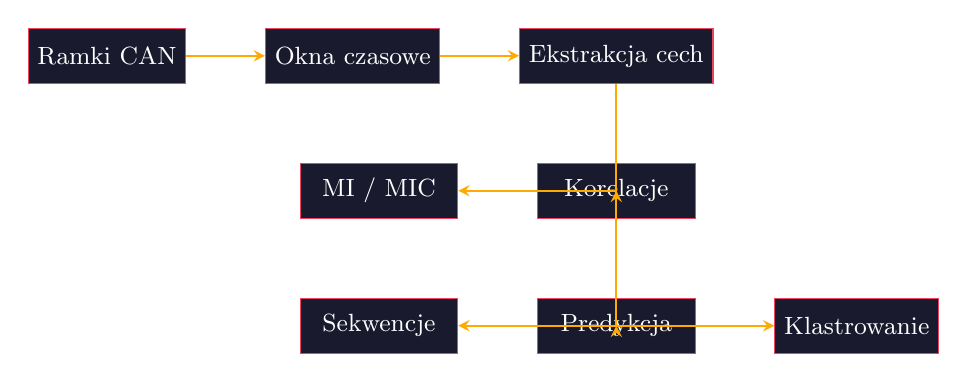
\begin{tikzpicture}[
  block/.style={rectangle, draw=accent, fill=codebg, text=white, minimum width=2cm, minimum height=0.7cm, font=\small},
  arrow/.style={->, >=stealth, thick, color=neonorange}
]
\node[block] (raw) {Ramki CAN};
\node[block, right=1cm of raw] (win) {Okna czasowe};
\node[block, right=1cm of win] (feat) {Ekstrakcja cech};
\node[block, below=1cm of feat] (corr) {Korelacje};
\node[block, left=1cm of corr] (mi) {MI / MIC};
\node[block, below=1cm of corr] (pred) {Predykcja};
\node[block, left=1cm of pred] (seq) {Sekwencje};
\node[block, right=1cm of pred] (clust) {Klastrowanie};
\draw[arrow] (raw) -- (win);
\draw[arrow] (win) -- (feat);
\draw[arrow] (feat) |- (corr);
\draw[arrow] (feat) |- (mi);
\draw[arrow] (feat) |- (pred);
\draw[arrow] (feat) |- (seq);
\draw[arrow] (feat) |- (clust);
\end{tikzpicture}
\caption{Potok analizy: od ramek do wyników.}
\label{fig:pipeline}
\end{figure}

\section*{Dodatek B – Struktura pliku DBC (uproszczona)}
\begin{lstlisting}[caption={Fragment pliku DBC}]
BO_ 1234 ExampleMsg: 8 Vector__XXX
 SG_ EngineSpeed : 0|16@1+ (0.5,0) [0|8000] "rpm" Vector__XXX
 SG_ Temperature : 16|8@1+ (1,-40) [-40|210] "degC" Vector__XXX
\end{lstlisting}

\end{document}